%%%%%%%%%%%%%%%%%%%%%%%%%%%%%%%%%%%%%%%%%
% Structured General Purpose Assignment
% LaTeX Template
%
% This template has been downloaded from:
% http://www.latextemplates.com
%
% Original author:
% Ted Pavlic (http://www.tedpavlic.com)
%
% Note:
% The \lipsum[#] commands throughout this template generate dummy text
% to fill the template out. These commands should all be removed when 
% writing assignment content.
%
%%%%%%%%%%%%%%%%%%%%%%%%%%%%%%%%%%%%%%%%%

%----------------------------------------------------------------------------------------
%	PACKAGES AND OTHER DOCUMENT CONFIGURATIONS
%----------------------------------------------------------------------------------------

\documentclass{article}

\usepackage{fancyhdr} % Required for custom headers
\usepackage{lastpage} % Required to determine the last page for the footer
\usepackage{extramarks} % Required for headers and footers
\usepackage{graphicx} % Required to insert images
\usepackage{lipsum} % Used for inserting dummy 'Lorem ipsum' text into the template
\usepackage{url} %For urls

% Margins
\topmargin=-0.45in
\evensidemargin=0in
\oddsidemargin=0in
\textwidth=6.5in
\textheight=9.0in
\headsep=0.25in 

\linespread{1.1} % Line spacing

% Set up the header and footer
\pagestyle{fancy}
\lhead{\hmwkAuthorName} % Top left header
\rhead{\firstxmark} % Top right header
\lfoot{\lastxmark} % Bottom left footer
\cfoot{} % Bottom center footer
\rfoot{Page\ \thepage\ of\ \pageref{LastPage}} % Bottom right footer
\renewcommand\headrulewidth{0.4pt} % Size of the header rule
\renewcommand\footrulewidth{0.4pt} % Size of the footer rule

\setlength\parindent{0pt} % Removes all indentation from paragraphs

%----------------------------------------------------------------------------------------
%	DOCUMENT STRUCTURE COMMANDS
%	Skip this unless you know what you're doing
%----------------------------------------------------------------------------------------

% Header and footer for when a page split occurs within a problem environment
\newcommand{\enterProblemHeader}[1]{
\nobreak\extramarks{#1}{#1 continued on next page\ldots}\nobreak
\nobreak\extramarks{#1 (continued)}{#1 continued on next page\ldots}\nobreak
}

% Header and footer for when a page split occurs between problem environments
\newcommand{\exitProblemHeader}[1]{
\nobreak\extramarks{#1 (continued)}{#1 continued on next page\ldots}\nobreak
\nobreak\extramarks{#1}{}\nobreak
}

\setcounter{secnumdepth}{0} % Removes default section numbers
\newcounter{homeworkProblemCounter} % Creates a counter to keep track of the number of problems

\newcommand{\homeworkProblemName}{}
\newenvironment{homeworkProblem}[1][Eric Ries: ``The Lean Startup" | Talks at Google]{ % Makes a new environment called homeworkProblem which takes 1 argument (custom name) but the default is "Problem #"
\stepcounter{homeworkProblemCounter} % Increase counter for number of problems
\renewcommand{\homeworkProblemName}{#1} % Assign \homeworkProblemName the name of the problem
\section{\homeworkProblemName} % Make a section in the document with the custom problem count
\enterProblemHeader{\homeworkProblemName} % Header and footer within the environment
}{
\exitProblemHeader{\homeworkProblemName} % Header and footer after the environment
}

\newcommand{\problemAnswer}[1]{ % Defines the problem answer command with the content as the only argument
\noindent\framebox[\columnwidth][c]{\begin{minipage}{0.98\columnwidth}#1\end{minipage}} % Makes the box around the problem answer and puts the content inside
}

\newcommand{\homeworkSectionName}{}
\newenvironment{homeworkSection}[1]{ % New environment for sections within homework problems, takes 1 argument - the name of the section
\renewcommand{\homeworkSectionName}{#1} % Assign \homeworkSectionName to the name of the section from the environment argument
\subsection{\homeworkSectionName} % Make a subsection with the custom name of the subsection
\enterProblemHeader{\homeworkProblemName\ [\homeworkSectionName]} % Header and footer within the environment
}{
\enterProblemHeader{\homeworkProblemName} % Header and footer after the environment
}
   
%----------------------------------------------------------------------------------------
%	NAME AND CLASS SECTION
%----------------------------------------------------------------------------------------

\newcommand{\hmwkTitle}{Eric Ries: ``The Lean Startup" | Talks at Google} % Assignment title
\newcommand{\hmwkAuthorName}{The Rising Tilde} % Your name

%----------------------------------------------------------------------------------------
%	TITLE PAGE
%----------------------------------------------------------------------------------------

\title{
\vspace{2in}
\textmd{\textbf{ \hmwkTitle}}\\
\vspace{3in}
}

\author{\textbf{\hmwkAuthorName}}
\date{} % Insert date here if you want it to appear below your name

%----------------------------------------------------------------------------------------

\begin{document}

\maketitle
\newpage
%----------------------------------------------------------------------------------------
%	PROBLEM 1
%----------------------------------------------------------------------------------------

% To have just one problem per page, simply put a \clearpage after each problem

\begin{homeworkProblem}

\textbf{Source:} 
\url{https://www.youtube.com/watch?v=fEvKo90qBns} \vspace{10pt} % Question


After graduating from Yale, Eric Ries worked as a software engineer at There, Inc. Due to an unfortunate failure, Ries left There to start another company, IMVU, Inc. IMVU was a social networking company that allowed people to create their own 3D avatars, meet new people, chat and inherited similar properties as Facebook now does. After stepping down as CTO, Ries left IMVU and became a venture advisor at Kleiner Perkins after leaving IMVU. This emerged as a turning point in his career.\vspace{10pt}

Despite having a strong background in computer science, Ries recognized a limitation in the way new product development is organized. He believed that entrepreneurship is management that fundamentally differs from general management and is measured by validated learning. Thus, enabling entrepreneurs to reiterate ideas and learn through a mechanism that enables them constantly assimilate new information from their past experiences.\vspace{10pt}

Ries, in his presentation, begins by describing what a startup is -``A human institution designed to create something new under conditions of extreme uncertainty". It has nothing to do with the size of the company, sector of the economy, or industry. When entrepreneurs are uncertain about their customers, it drives them to research more. A startup's goal should be to constantly understand the needs of its customers, the products they want. By doing so, it allows the business to build a sustainable model because they can tailor to the customer's needs.\vspace{10pt}

``The biggest waste product development faces today is not building things inefficiently but building things efficiently that nobody wants." For example, with the emergence of Web 2.0 in 2006, several startups appeared to be promising. But three years later, a majority of these startups either failed or were absorbed by larger companies. Very few came to be known to be as ``Success Stories". Ries outlined success stories as not those who made money, but companies that ``succeeded in living up to the aspirations, dreams, time, talent and energy of the founders, investors, and their employees". \vspace{10pt}

Project management methodologies such as agile, extreme programming and waterfall depend on the customer to give an authoritative, definite answer to design questions. Without a solution to the product at best, as a startup, we have a theory or hypothesis about what the customer may want. ``If you don't know who your customer is, you don't know what quality means". This here is the fundamental problem of lean startups.\vspace{10pt}

The specifications of the product remain insignificant to the customer if the product doesn't meet appropriate quality. Furthermore, the customer `doesn't care' if the product doesn't meet his/her needs. The issue is to construct a sustainable business model around a particular product. A startup could boast about finishing a product on time and within budget while still ``achieving failure". With an oversaturated market, it is clear that the question isn't whether ``it can be built", but ``should it build". ``Everything that we do should be gauged to be decided by whether the customer cares that we do it." \vspace{10pt}

Most successful startups had ludicrously bad ideas at the beginning. The fascinating part about entrepreneurs of such businesses is that rather than preserving indefinitely in an event of a failure, they pivoted. Similar to an analogy in basketball, ``one foot firmly rooted, while changing one other thing about the business". Startups should focus on reducing the time between pivots to decrease the chances of failure before the business is exhausted of its resources. Furthermore, startups shouldn't be misled by fact that the amount of money remaining reflects the ability of the startup to survive, but instead, the emphasis should be on the number of opportunities are left to pivot. \vspace{10pt}

Steve blanks introduced a process known as iterative development for customers. This method is used to figure out your customer segment while merging this model in parallel with agile development. This accommodates agile development by providing a feedback loop of learning and discovery. Hence, establishing validated learning. \vspace{10pt}

There needs to be a system to rigorously assess whether the product being built is sustainable or not. For example, Ries realized if he had built a photo mockup of IMVU initially, he would have saved roughly six months of development time. But would the six months be regarded to as a waste of time? No, because eventually, they were able to recognize the importance of customer feedback at an earlier stage. This elucidates the concept of validated learning, which highlights that failure is of significant importance to startups or sometimes the only option. What did IMVU learn? - those customers weren't looking for interoperability or an add-on for their IM clients, but instead were looking for a new way to find friends. \vspace{10pt}

This allows us to introduce the concept of a minimum viable product. An MVP states what really needs to be in the first version. It helps decide and narrow down only what is necessary to learn and condemns everything else as extraneous.  As a software company, this is what the core components look like. \vspace{10pt}

\begin{center}
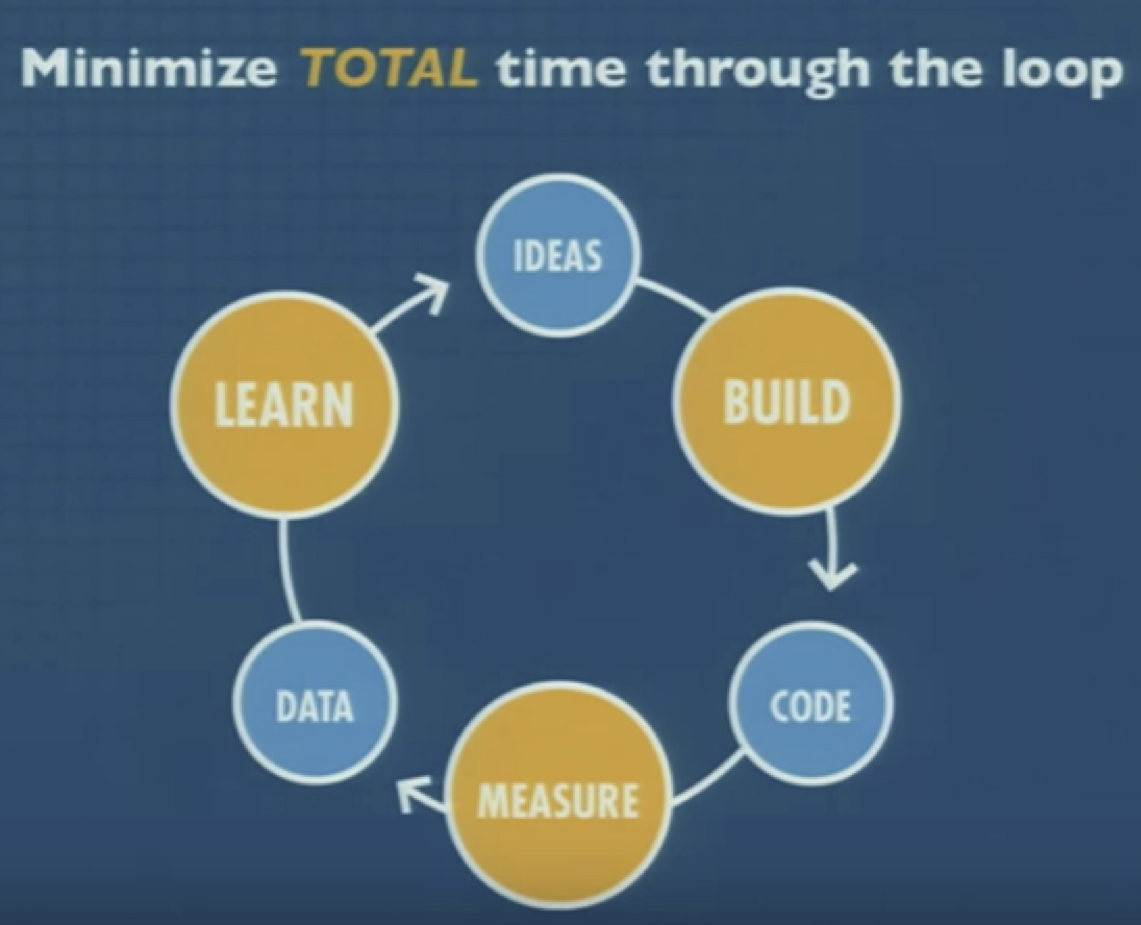
\includegraphics[width=0.5\columnwidth]{example_figure} % Example image
\end{center}

Customers help turn this idea into code.  A pivot is one major turn in this feedback loop. As the aim of a company should be to minimize the time through this loop. For example, a fatal flaw in IMVU's product was that they created their product for seven IM client rather than creating for one and then testing its accountability.\vspace{10pt}

Another major aspect in lean startups is innovation accounting. This system allows portraying entrepreneurship success on a quantitative basis. Accounting shouldn't be misinterpreted here as a process that includes processing of financial information but rather a communication that drive accountability across departments. Instead of focusing on product milestones and gross numbers, there are three learning milestones - establish the baseline, turn the engine and pivot or preserve. \vspace{10pt}

The baseline of a company can be established by building a minimum viable product and measure how customers behave with regards to the product. Regardless of how bad the baseline, this should be regarded as progress as the startup would have formulated a basic idea of what the customer wants. The next step is to convert the ``horrible" baseline to the ideal conversion numbers in your business plan. Instead of getting to the point of diminishing returns, schedule a meeting in advance to decide whether to pivot or persevere. In conclusion, train your judgment to be better over time, hence, allowing yourself to pivot earlier (with practice). Understanding the customer that thus drives the sustainability of your product.\vspace{10pt}

\end{homeworkProblem}

\end{document}
